%!TEX root = ../main.tex
\documentclass[a4paper,oneside,12pt, class=Latex/Classes/PhDthesisPSnPDF, crop=false]{standalone}
\usepackage{setspace}
\begin{document}
\doublespacing
\chapter{Observing in the optical regime}
\label{chap:obs}

%\color{red}To do list: recheck carefully, layout\color{black}

Astrophysicists face the challenge of not being able to set up and control their experiments. The universe is our laboratory, but all we can do is see or detect the results while often not knowing the exact setup of the experiment. Models are made to explain and predict the behaviour of planets, stars, and galaxies, but ultimately, observations are needed to compare against and test our models. My work relies heavily on observational data, and in this chapter I will introduce the different types of observations that are used throughout this thesis (section~\ref{observation_types}), telescopes and instruments that are used to obtain these observations (section~\ref{telescopes}), and a quick overview of how to calibrate the raw images and extract useful data (sections~\ref{calibration} and~\ref{reduction}). I will also give a general overview of what to consider when planning observations in section~\ref{considerations}.


\section{Types of obeservations}
\label{observation_types}
All optical observations are, in essence, images taken by a camera. Light falls onto a pixel on the detector (a charge-coupled device, CCD) and frees some amount of electrons. If more light hits the pixel, more electrons are freed. At readout these electrons are counted per pixel, or group of pixels if binning is applied, and turned into a digital number called a count or analog-to-digital unit (ADU). The gain (e$^-$~/~ADU conversion rate) is a unique property of each readout channel, and sets the conversion rate between the measured number of electrons and the resulting value that is stored. One of the main advantages of CCDs is their low read noise levels (mean e$^-$ added to a pixel upon readout), with modern CCDs having a read noise level of only a couple of electrons. Observations have contributions from different noise sources, but as long as the total count rate is in the linear regime of the CCD, there is a linear relation between the received flux and the final count. By using calibration images, it is then possible to calculate the observed flux \citep{CCD_handbook}. Section~\ref{calibration} explains the different types of calibration images, and section~\ref{reduction} explains their usage in image reduction.


\begin{figure}
    \centering
    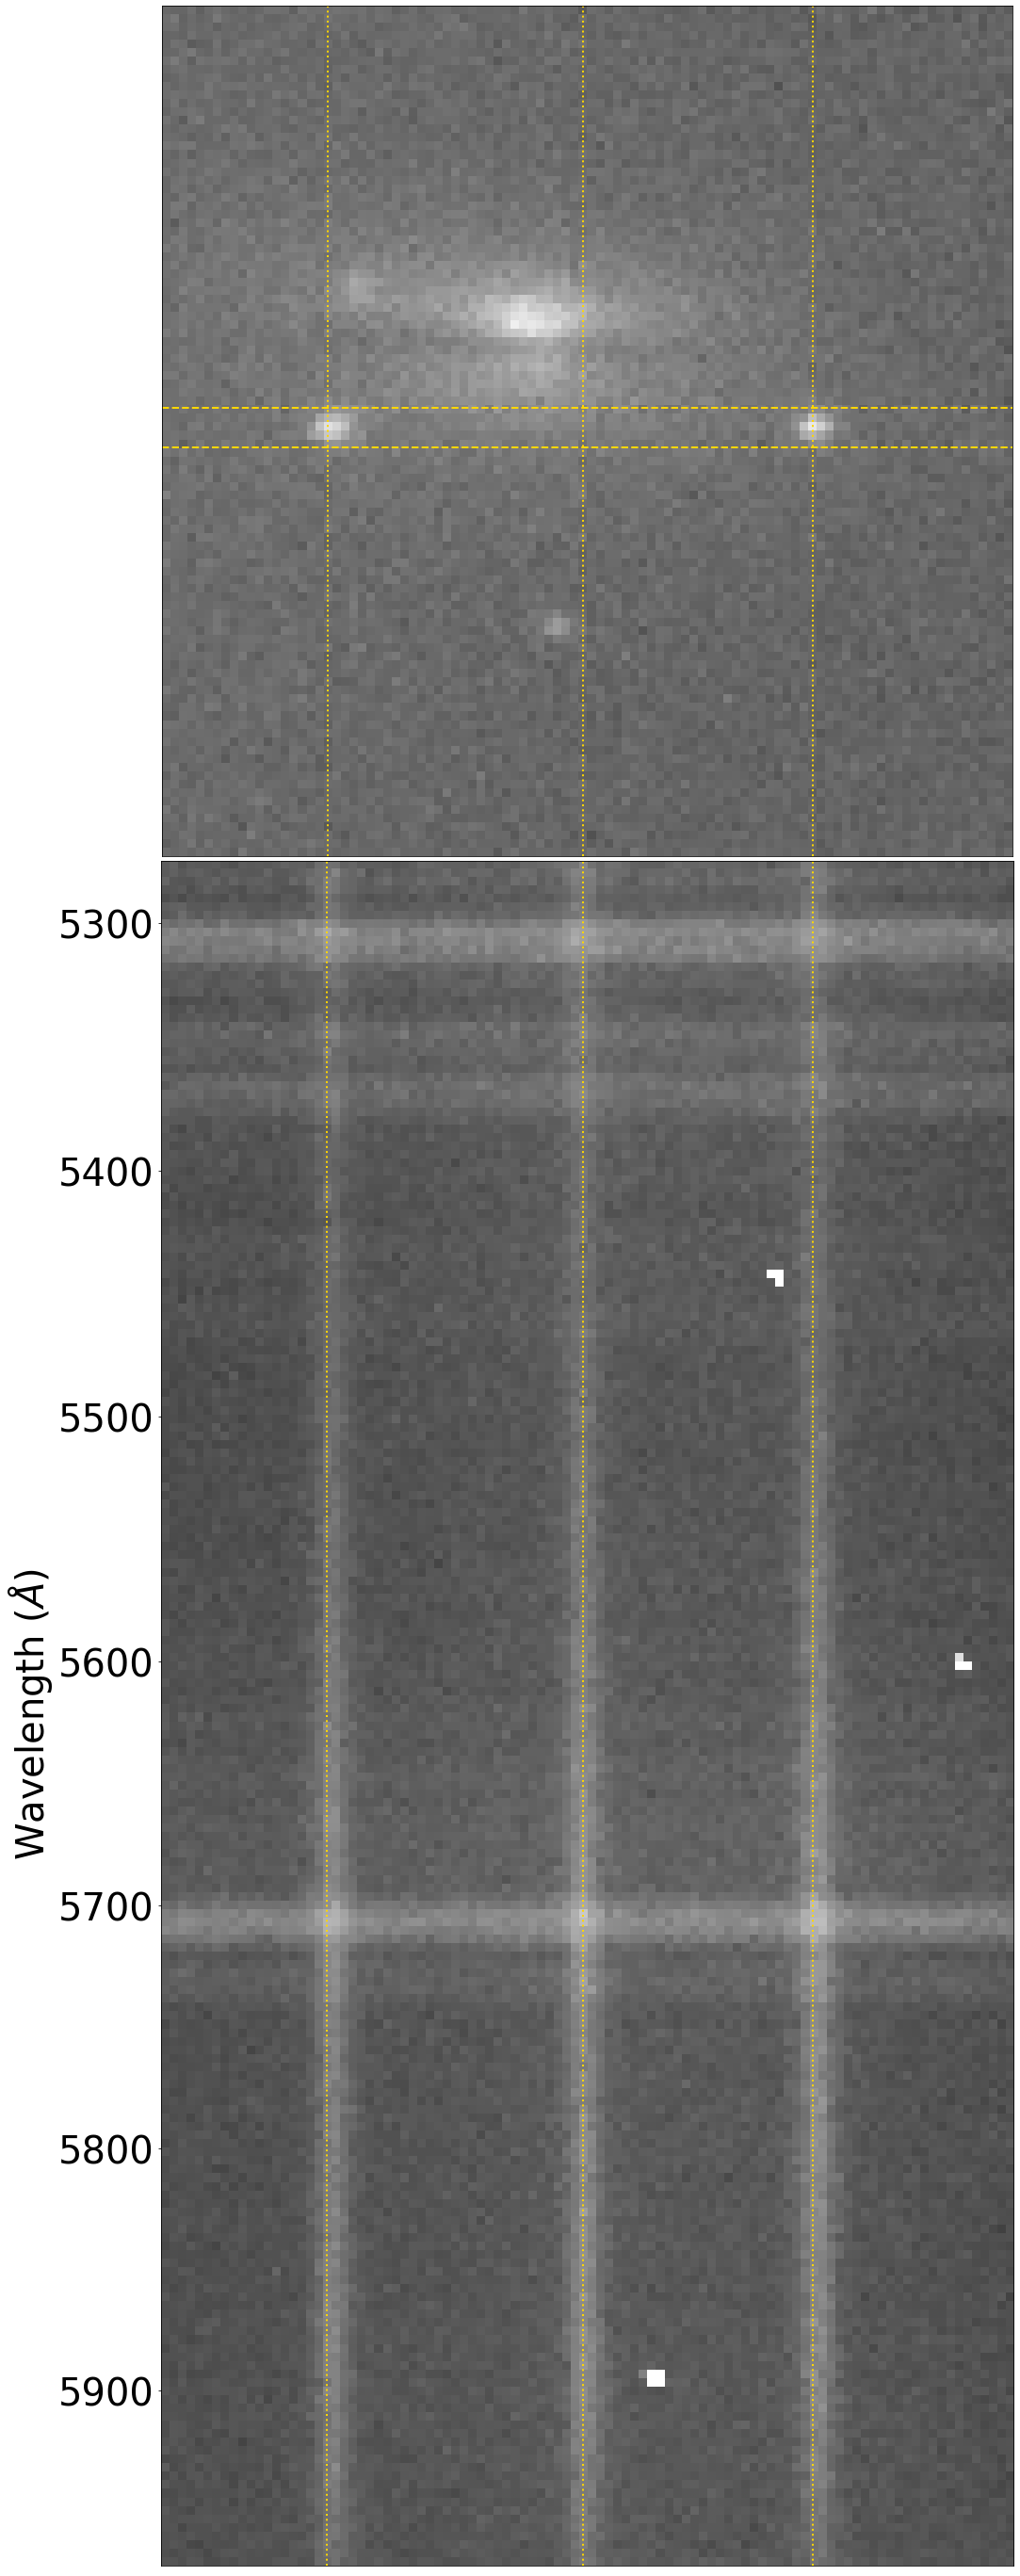
\includegraphics[height=0.83\textheight]{../Images/chapter_2/phot_and_spec_example.png}
    \caption{Image and partial spectrum of SN~2024nqr (left) and SN~2024pgd (right), two SNe~Ia simultaneously active in the same galaxy. The image was taken without a filter and used to align the 1.0$\arcsec$ slit (horizontal dashed lines) over both SNe. The resulting spectrum, taken with grism~\#4, shows three traces as white vertical stripes. The outer two line up with the two SNe, while the middle trace is from the edge of the host galaxy, which is in the slit (vertical dotted lines for guidance). The horizontal lines in the spectrum are sky lines coming from atmospheric emission, and the white spots in the spectrum are due to cosmic rays. This data was taken with NOT+ALFOSC on the night of 28 July 2024 while testing an experimental rapid response mode (RRM, credit: Samuel Grund S\o rensen).} %Just going to assume the AT/SN thing is eventually fixed
    \label{phot_spec_example}
\end{figure}

\subsection{Photometry}
Photometry is one of the simplest observing modes, as it is just taking a photo of a part of the sky. The top of Fig.~\ref{phot_spec_example} shows a raw photometric image taken with ALFOSC on the Nordic Optical Telescope (NOT) without using a filter. The images are monochromatic, meaning they only have a value for the light intensity received per pixel. To obtain colourful images multiple observations have to be made using different filters, which are then combined to represent different colours in the final image.

Faint objects can be observed by increasing the exposure time in a single image, or by stacking multiple images together to increase the effective exposure time. Stacking images can be useful for, e.g., reducing cosmic ray interference, avoiding overexposure of a bright source close to a fainter target, or constructing time series. When stacking images, it is common practice to dither the telescope: applying a small offset between exposures to ensure that the target hits a different part of the CCD to avoid issues with bad pixels ruining otherwise good observations. While this decreases the effective size of the fully stacked image, as long as the edges are not needed there is no issue \citep{Stacking_I, Stacking_II}.

\subsection{Spectroscopy}
Spectroscopy goes one step beyond just taking a photo. In slit spectroscopy, instead of a filter to select a wavelength range to observe, now a slit restricts the observable region of the sky to a narrow band along one axis of the detector (e.g. horizontal). After the slit, the light hits a grating or grism (a grating and prism combined), which diffracts the light based on wavelength across the second axis of the detector (vertical). The rule density on the grating or grism dictates the wavelength spread of the light: the more rules per unit distance, the bigger the dispersion, and the higher the spectral resolution of the resulting image. The tradeoff is that a smaller part of the spectrum can be observed at a time, and there is less light being received per pixel which reduces the SNR unless the exposure time is increased to account for this. Any point-like source that is observed becomes a line in the spectral direction, called a trace. Extended sources create extended traces.

There is some freedom in choosing the orientation of the slit. This is called the position angle of the slit. If there are multiple targets near each other, and they can be in the slit at the same time, the required position angle can be calculated from the two target positions. If there is a single target to be observed, the position angle can be anything, but usually the parallactic angle is chosen. In this orientation the slit is perpendicular to the horizon, and prevents losses from differential diffraction (different colours diffracting differently when entering the atmosphere at an angle, \citealt{diff_refrac_atmosphere}). The trace will only be slightly diagonal on the CCD.

The bottom panel of Fig.~\ref{phot_spec_example} shows a section of the spectrum taken of the SNe in the top panel image. The two SNe are drawn out into vertical traces, and a third trace belonging to the edge of the host galaxy can be seen in the middle. The horizontal lines are sky emission lines, and while these can technically be used to estimate the conversion from pixel position to wavelength, standardized arc frames will result in a much better wavelength calibration (see section~\ref{reduction}).


\section{Telescopes}
\label{telescopes}
Most of the data used in this thesis comes from the Zwicky Transient Facility (ZTF), and follow-up observations have been made using the Nordic Optical Telescope (NOT), and the Gran Telescopio CANARIAS (GTC), which will be introduced below. Some additional data comes from other sources, which are listed for completeness. The same filter names (\ztfg\ztfr\ztfi) are used for filters at different telescopes,  which have slight differences. In the rest of this thesis I will use \ztfg\ztfr\ztfi\ to refer to the ZTF filters, unless specified otherwise.

\subsection{Zwicky Transient Facility}
\label{ZTF}
The Zwicky Transient Facility (ZTF, \citealt{ZTF_Surveys_Scheduler, ZTF_overview_and_1st_results, ZTF_Science_Objectives, ZTF_Instrumentation, ZTF_Observing_System}) is an optical large-sky survey observing the entire northern night sky above Dec $\approx -30$\degree\ every 2 to 3 nights in three broadband optical filters \ztfg~($\lambda_{eff} = 4\,746.48$ \AA), \ztfr~($\lambda_{eff} = 6\,366.38$ \AA), and \ztfi~($\lambda_{eff} = 7\,829.03$ \AA), which are similar to the well-known SDSS \ztfg\ztfr\ztfi\ filters. The efficiency of these filters is plotted as a function of wavelength in Fig. \ref{Optical_elements_plot}. The survey saw its first light in October 2017 and it formally began scientific operation in March 2018, and has been running continuously until the time of writing this thesis.

The observations are made using the $48\arcsec$ aperture Schmidt-type design Samuel Oschin Telescope, which is based at the Palomar Observatory in Southern California. Each exposure is 30 s long, can go a limiting magnitude of $\sim20.5$ mag, and covers an area of $\sim47$ deg$^2$ at a resolution of $1.01\arcsec$ per pixel. The camera is divided into a $4\times4$ grid of CCDs, each of which has four readout channels called quadrants. This results in each observation producing 64 separate images, each with its own readout channel identifier (rcid). Similarly, the observed region of the sky is divided into different telescope pointings called fields to ensure that the same region of the sky is observed in the same way each time, aiding with the reduction of the data. This results in each combination of filter, field, and rcid being a set of observations of a particular part of the sky using a specific setup.

\begin{figure}
    \centering
    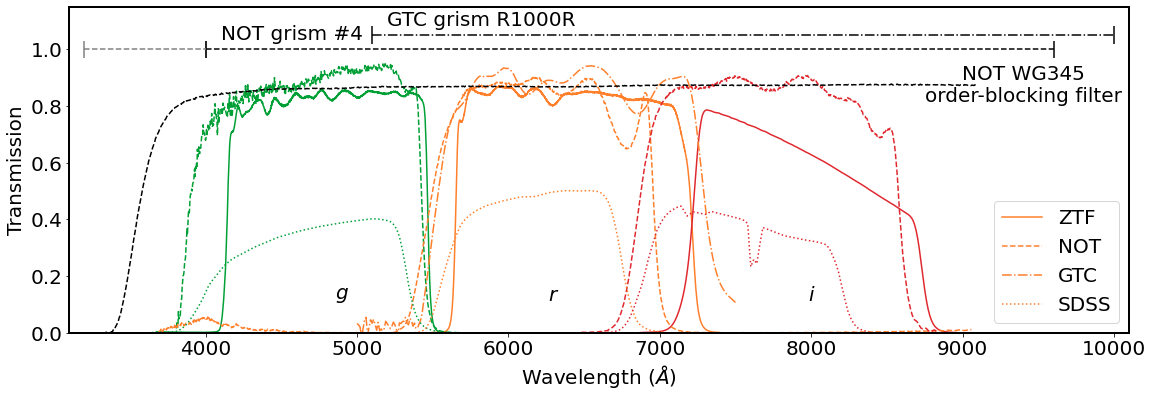
\includegraphics[width=\textwidth]{../Images/chapter_2/transmissions.png}
    \caption{Throughput as a function of wavelength of the different filters used to gather the bulk of the data in this thesis. \ztfg\ filters are shown in green, \ztfr\ in orange, \ztfi\ in red, and the different telescopes are shown with different line styles (Continuous for ZTF, dashed for NOT, dot-dashed for GTC). The SDSS filter transmissions (dotted lines) are shown for comparison. The black dashed line is the WG345 order-blocking filter that was used for some spectroscopic observations taken with the NOT. For the grisms only the wavelength ranges are shown, not their efficiency at each wavelength.}
    \label{Optical_elements_plot}
\end{figure}


\subsection{Nordic Optical Telescope}
\label{NOT}
The Nordic Optical Telescope (NOT)\,\footnote{\url{https://not.iac.es}} is a 2.56 m telescope located at Observatorio Roque de Los Muchacos in La Palma, Spain, at an elevation of 2382 m above sea level. It hosts several instruments for observing in the optical and near-infrared, both for imaging and spectroscopy. The \textit{Alhambra Faint Object Spectrograph and Camera} (ALFOSC) was used to obtain the data used in this thesis. I will only discuss the parts relevant to this thesis, further details on this instrument and details on the other instruments can be found on the NOT website.

ALFOSC is a versatile instrument mounted in cassegrain and can be used for imaging, spectroscopy, and (spectro)polarimetry. As there are several wheels equipped to hold a variety of optical elements, the instrument can switch quickly between different setups between observations. The images can cover up to $6.4\arcmin\times6.4\arcmin$ per exposure at a resolution of $0.2138\arcsec$ pixel$^{-1}$. In this thesis \ztfg~($\lambda_{cen} = 4\,800$ \AA), \ztfr~($\lambda_{cen} = 6\,180$ \AA), and \ztfi~($\lambda_{cen} = 7\,710$ \AA) are used for photometry. For spectroscopy grism \#4 is used to split the light vertically, together with a horizontal $1.0\arcsec$ slit if the seeing was $\leq1.3\arcsec$ or a horizontal $1.3\arcsec$ slit if the seeing was $\geq1.3\arcsec$. Grism \#4 has a resolution of 3.3~\AA~pixel$^{-1}$ and a wavelength range from 3\,200 \AA\ to 9\,600 \AA, but as the response at short wavelengths is poor, the spectra used in this thesis are cut at 4\,000 \AA. For some spectra an order-blocking filter (WG345) is used as well to avoid second-order diffracted blue light overlapping with first-order diffracted red light on the detector. The transmission curves of the filters and wavelength range of the grism are shown in Fig.~\ref{Optical_elements_plot}.


\subsection{Gran Telescopio CANARIAS}
\label{GTC}
The Gran Telescopio CANARIAS (GTC)\,\footnote{\url{https://www.gtc.iac.es}} is a 10.4 m telescope at Observatorio Roque de los Muchachos in La Palma, Spain, and is the largest optical/near-infrared telescope on the island. Its primary mirror is made up of 36 hexagonal pieces, creating an effective collection area of 73 m$^2$, ideal for observing very faint targets. The GTC can host up to six instruments at a time in various focal positions, allowing for a large variety of observations to be made. One of the most commonly used instruments is OSIRIS+, the upgraded version of OSIRIS: the \textit{Optical System for Imaging and low-Intermediate-Resolution Integrated Spectroscopy}.

OSIRIS+ has an unvignetted field-of-view of $7.8\arcmin\times7.8\arcmin$ at a resolution of $0.254\arcsec$~pixel$^{-1}$. Since the standard readout has $2\times2$ binning, the resolution can be increased to $0.127\arcsec$~pixel$^{-1}$ if so desired. Like ALFOSC, this instrument is also built to easily switch between different setups between observations. For photometry the \ztfr~($\lambda_{cen} =6\,410$ \AA) filter is used in this thesis, and for spectroscopy the R1000R grism with a $1.0\arcsec$ vertical slit is used. R1000R splits the light horizontally over the detector with a range of 5\,100 \AA\ to 10\,000 \AA\ with a resolution of 2.62 \AA\ pixel$^{-1}$. These filter transmission curve and grism wavelength range are shown in Fig.~\ref{Optical_elements_plot}.


\subsection{Other observations}
Small amounts of data coming from other telescopes and surveys are presented in this thesis as well. This includes a follow-up observation of SN~2019ldf in section \ref{sec:late_time_cand} in \ztfg\ and \ztfr\ using the \textit{ESO Faint Object Spectrograph and Camera version 2} (EFOSC2, \citealt{EFOSC2}) imaging spectrograph on the ESO New Technology Telescope (NTT) in La Silla, Chile as part of the extended Public ESO Spectroscopic Survey of Transient Objects+ (EPESSTO+, \citealt{PESSTO}).

To complement ZTF data of several SNe, in chapter \ref{chap:pre-ZTF_search} optical photometry from the Panoramic Survey Telescope and Rapid Response System (Pan-STARRS, \citealt{Pan-STARRS1}), (intermediate) Palomar Transient Factory (PTF, \citealt{PTF_1, PTF_2}, iPTF, \citealt{iPTF}), All Sky Automated Survey for SuperNovae (ASASSN, \citealt{ASASSN_paper1, ASASSN_catalog}), Asteroid Terrestrial-impact Last Alert System (ATLAS, \citealt{ATLAS}),  and \textit{Global Astrometric Interferometer for Astrophysics} (Gaia, \citealt{Gaia}) are used. In chapters \ref{chap:DR2_search}, \ref{chap:pre-ZTF_search}, and \ref{chap:Real-time} near-infrared photometry from the \textit{Wide-Field Infrared Survey Explorer} (WISE, \citealt{WISE}) is used as well.

For difference imaging, data from the DESI Legacy Imaging Surveys Data Release 9 \citep{DESI-Legacy_Imaging_Surveys} were used as references for the SN 2019ldf followup data, and data from Pan-STARRS and the Sloan Digital Sky Survey (SDSS, \citealt{SDSS-I-II, SDSS_DR4, SDSS_telescope, SDSS_Spectograph}) were used as reference images for followup observations taken with the NOT and GTC.


\section{Calibration images}
\label{calibration}
Before observations can be used for science, the images need to be calibrated. This is done using different types of calibration images, each of which measures and corrects for different effects of the telescope and detector. Table 4.1 from \citet{CCD_handbook} has an overview of the different types of calibration images used for photometry. Usually, calibrations are taken during the day or twilight so no valuable observing time is lost. It is standard practice to take multiple calibration images and use an odd number in the reduction to find median values and remove interference from e.g. cosmic rays.


\subsection{Bias}
The first type of calibration image is the bias, which is made by reading out the CCD without exposing. The resulting image contains the number of counts that will be in every exposure regardless of what has been observed or with what exposure time. In other words, measuring the bias can be thought of as measuring the offset to correct for in every other image, and the underlying noise level in each frame.


\subsection{Dark}
Any detector that is not at a temperature of 0 K will have some amount of noise due to thermal effects. This can free electrons in pixels over time, creating a dark current and increasing the noise over time. The effect can be measured by exposing for the same amount of time as the science images that were taken but without letting any light hit the CCD. This is called a dark frame.

As this is a thermal effect, it can be reduced to negligible amounts by cooling the instrument. This saves precious observing time, as otherwise dark frames would ideally have to be taken at the same temperature as the target was observed, which is easiest to do directly after the science exposure. By cooling the detector with e.g. liquid nitrogen, this noise source can be avoided instead of having to correct for it, saving time and the amount of images that need to be taken in the process.


\subsection{Flatfield}
The amount of light that the telescope receives is converted into a digital number, but there is no guarantee that this conversion rate is the same for each pixel. This can be due to intrinsic differences between the pixels, or outside effects such as dust reducing the amount of light received on a part of the detector. To correct for this, an evenly illuminated field has to be observed, resulting in an image called a flat or flatfield. By ensuring that each pixel receives the same amount of light, the different counts will reflect the varying responses per pixel.

Any evenly illuminated object can be used for this, such as the inside of the telescope dome to create dome flats. A more perfect evenly lit source, however, is the sky, and by using this, sky flats can be taken. While it is usually too bright during the day causing the CCD to saturate even with the narrowest filter and shortest exposure time, there is a window during twilight where the sky is darker but not dark enough to observe stars yet, perfect for taking flats. As a general rule, narrowband filters need a brighter sky, and in the evening these need to be done before the broadband filters. After that, assuming similar efficiencies between filters, blue filters need brighter skies than red filters, forcing a specific order in which the sky flats need to be taken during the short window when this is possible. Of course, if flats are taken in the morning, the order has to be reversed.


\subsection{Arc}
In spectroscopy one of the axes has the lowest wavelength at one end and the highest wavelength at the other end of the image. To know where each wavelength falls on the detector, arc frames are needed. These are taken by observing a lamp filled with a known set of elements (e.g. He, Ne, or TH and Ar). The wavelengths of the emission lines are known very precisely, and by matching these with the observed lines in the arc image a pixel-to-wavelength conversion can be found, called the wavelength solution.

Usually, arcs can be taken during the day when the telescope is idle. However, in some cases the mechanical flexure of the telescope, caused by it being in a different position during observing, can introduce an uncertainty in the wavelength calibration unless an arc is taken with the telescope in the same position as for the target. In these cases an arc is usually taken directly before or after the target is observed, or between exposures of the target \citep{CCD_handbook}.


\section{Reduction}
\label{reduction}
After all observations have been taken, it is time to analyze them. A thorough overview of this can be found in \citet{Image_processing}. The first step is to reduce the raw data into the required format to work with. After that, additional analysis techniques can manipulate the reduced images directly or the data that has been extracted from them. The response function of a detector can be written as

\begin{equation}
	R_{ij}(f, t, \lambda) = B_{ij} + D_{ij}(t) + F_{ij}(\lambda) \times f \times t,
	\label{CCD_response}
\end{equation}

where $R_{ij}$ is the CCD response of pixel $i,j$ as a function of the integrated flux of the target $f \times t$ during the exposure which lasted a time $t$. The goal is to measure the flux $f$, which requires knowing and correcting for the bias level $B_{ij}$, dark current $D_{ij}(t)$, and pixel response $F_{ij}(\lambda)$. Each type of calibration image is used to measure one of these values. Note that it is assumed that there are no cross or higher order terms in Eq.~\ref{CCD_response}. In other words, the CCD is in its linear regime. When a pixel receives too much light and gets close to saturating, it is no longer in its linear regime and more terms appear in Eq.~\ref{CCD_response}, making it much more difficult or even impossible to measure the observed flux.


\subsection{Bias, dark, and flat corrections}
Using the calibration images from section~\ref{calibration}, the raw science images can be reduced to something a flux level can be measured from. 

First, the master bias frame is created and subtracted from every other image. As both $f$ and $t$ are 0, the bias measures $B_{ij}$ directly and can then immediately be removed.

Secondly, the dark frames measure $D_{ij}(t)$ for a specific $t$, but the master dark frame  can only be used on science observations with the same exposure time. Alternatively, it is possible to subtract $B_{ij} + D_{ij}(t)$ in a single step by not separating out the bias term using bias images first.

Finally, every science image is divided through the normalized master flat to equalize the pixel responses. There is still a factor $F(\lambda)$ present as the detector efficiency is wavelength-dependent, but that value is now independent of the pixel position, allowing values from across the CCD to be compared.

\subsection{Cosmic-ray removal and image stacking}
At this point it is often good practice to run a cosmic-ray removal algorithm to remove this source of noise as much as possible. This can be done using, for instance, L.A.Cosmic \citep{lacosmic}, which I used through Astro-SCRAPPY \citep{astroSCRAPPY} when reducing follow-up photometry of several objects in this thesis.

If multiple images are taken of the same field or object they can be stacked to reduce background noise and increase the SNR of the observed objects. Sometimes the observations have been taken with dithering to avoid the same objects being on the same pixels in every exposure, which has to be taken care of to make sure that the images are stacked correctly.

\subsection{Standard star calibration}
Filters are never 100\% transparent at any wavelength, and the CCD responds differently to different wavelengths as well. To correct for this, one last type of calibration image is used: the standard star. This was not mentioned in section~\ref{observation_types} as observing a standard star is exactly the same as observing the actual science target. The only difference is that the expected result of the observation is known and can be used to correct for the wavelength-dependent efficiency of the instrument.

With photometry, the observed brightness can be measured for each star in the image to get a list of instrument magnitudes. The relative differences between the magnitudes of objects are correct, but there is still an absolute offset across all objects. This is corrected by finding the offset using the standard star. If the filter is commonly used, there is a good chance many stars in the field have known magnitudes in that filter, which can be used for calibration instead of a dedicated standard star.

In spectroscopy, the arcs are used to find the wavelength solution for the spectra, after which the trace from the standard star can be extracted and divided by the known spectrum of the star to obtain the sensitivity function of the detector $F(\lambda)$. The trace of the target can be extracted as well to get its spectrum, which can then be flux-calibrated using the sensitivity function. In some cases, only a relative sensitivity function is known, resulting in a calibrated spectrum in an unknown flux unit. In these cases, properly calibrated photometry of the object can be used to flux-calibrate the spectrum by integrating the spectrum over the filter transmission curve.


\subsection{(Forced) photometry}
The two most common methods to measure flux from a source in an photometric image are PSF photometry and aperture photometry. A good explanation of these can be found in \citet{Photometry_techniques}. PSF stands for point spread function, and with this method a function is fitted to model the source. This function describes how an infinitely small point of light is spread over the detector, and through its spatial size and peak value the flux of the light source can be measured. Aperture photometry sums up the signal in a given radius around the source centre and subtracts the contribution from the background in the same region.

Large surveys such as ZTF observe the night sky to find new transients and monitor known ones. Difference imaging is used to subtract constant sources and reveal active transients, as these are the main sources that should be left in the difference image along with solar system objects that move across the sky. Figure \ref{diff_im_example} shows an example of a reference image, a science image, and the resulting difference image. A historically popular algorithm for difference imaging is High Order Transform of PSF ANd Template Subtraction (\textsc{hotpants}, \citealt{HOTPANTS})\,\footnote{\url{https://github.com/acbecker/hotpants}}, which is used for image subtraction in section \ref{sec:late_time_cand}. Besides this, there are other algorithms as well. For instance, ZTF uses \textsc{zogy} \citep{ZOGY}\,\footnote{\url{https://github.com/cenko/ZOGY}}, and in chapter \ref{chap:Real-time} \textsc{autophot} \citep{Autophot}\,\footnote{\url{https://github.com/Astro-Sean/autophot}} is used to subtract reference images from follow-up observations obtained with the NOT and GTC.

\begin{figure}
    \centering
    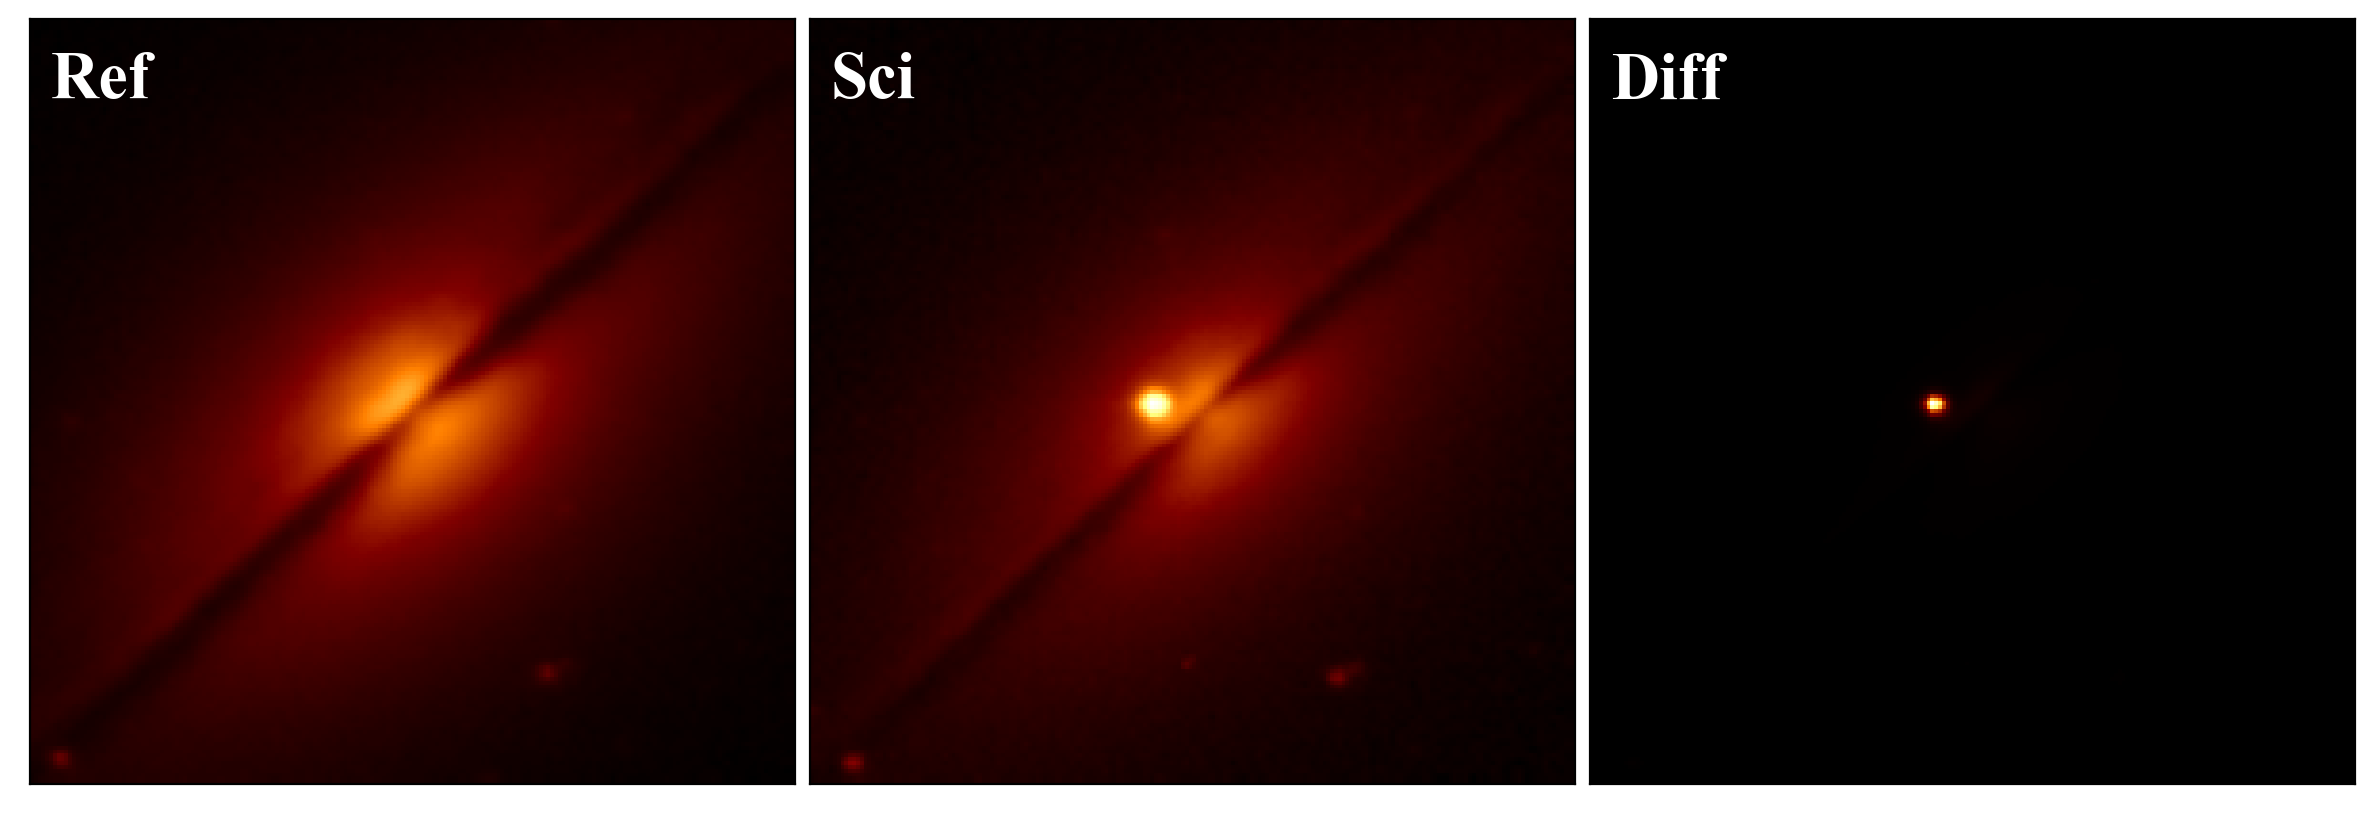
\includegraphics[width=\textwidth]{../Images/chapter_2/diff_im_SN2021rhu.png}
    \caption{Example of an \ztfr-band reference image of NGC 7814, the science image of the same region, and the resulting difference image with the host galaxy removed and only the transient (SN~2021rhu, SN Ia-86G) remaining. (Credit: Luke Harvey)}
    \label{diff_im_example}
\end{figure}

Through PSF photometry the location and strength of each source in the image is determined. These are then compared to the locations of known sources to separate new from known ones. Each location has however been observed for the entire duration of the survey, which means that it is also possible to measure the flux of a known transient before and after it was visible in the images and create a light curve for the full duration of the survey.

This is called forced photometry, because the PSF function is forced to center on a specific location instead of finding the best-fitting position for the centroid. All ZTF light curves that are used in this thesis have been obtained through \textsc{fpbot} \citep{fpbot}\,\footnote{\url{https://github.com/simeonreusch/fpbot}}, which uses forced photometry. When there is nothing but noise at that location, the measured flux will be 0 within the error. When there is a source at the target location, it will be measured, but if the source is not at the centre of the PSF, the fit will have trouble converging, resulting in a large uncertainty. Artefacts such as cosmic rays, imperfectly subtracted difference images, or light bleeding effects from saturated bright nearby stars can also affect the accuracy of the photometry measurement.


\section{General considerations for observing}
\label{considerations}
During my PhD I have spent two years doing observational studentships in La Palma. The first year was with the Isaac Newton Group of Telescopes (ING) and the second year with the NOT. I gained first-hand experience with the specifics of observing in the optical regime and the considerations that come with it. I will briefly go over these in this section. These studentships also gave me the unique opportunity to quickly follow up on interesting transients, which was very valuable for the objects I will discuss in chapter \ref{chap:Real-time}.


\subsection{Location}
Although this is usually already done before constructing a telescope, the first thing to consider is the observing location. When purely aiming for the best observations possible, there are three main things to consider when choosing where to observe from:
\begin{itemize}
    \item {Weather: Clear, stable sky conditions for most nights throughout the year, and low atmospheric distortion (e.g. seeing) are vital to ensure good quality data on a regular basis. Low-hanging clouds can be avoided by being high above sea level, while simultaneously decreasing the amount of air light has to travel through to reach the detector, decreasing atmospheric influence.}
    \item {Light pollution: Darker skies allow for observations of fainter objects. Even the presence of a (partially) illuminated moon significantly changes the depth that can be reached with the same exposure time. Many observatories have (inter)national laws to control the amount of light pollution and ensure that good quality data can be obtained.}
    \item {Target observability: The target location needs to be reachable by the telescope to be observable. The closer to zenith an observation is made, the less atmosphere between the target and the telescope. The atmosphere reduces the data quality through turbulence (seeing), broadband absorption (clouds, dust), narrowband interference (tellurics, sky lines), and differential diffraction, among others.}
\end{itemize}

Ideally, observatories should be located on top of high mountains in areas with stable and clear weather with as small a nearby population as possible, while still being accessible enough for transporting materials and observing staff. One of the best locations in the world that meets these requirements is Roque de los Muchachos on La Palma, a small Spanish island in the Atlantic Ocean off the coast of Morocco. At around 2300 m above sea level, the telescopes are built on the highest peak of the mountain, far from most communities on the island that are much closer to sea level, and the temperate climate ensures good sky conditions for most nights around the year. On top of that, in 1988 the government put the so-called "Law of the Sky" in place to minimize light pollution, e.g. by limiting the use of street lights and restricting flight paths over the island \citep{LP_Sky_law}.


\subsection{Telescope, instrument, observation type, and setup}
Depending on the type of observations and the brightness of the target, there is a choice of what hardware to use. Telescope, instrument, observation type, and desired setup(s) have to be considered together, as some choices will affect other ones.

Bigger telescopes can observe fainter targets, but it is also more difficult to obtain observing time. On the other hand, smaller telescopes are less oversubscribed (a measure of requested versus available observing time) but are more limited in observation depth, even with long exposure times.

Secondly, different instruments, which are often telescope-specific, have different observing capabilities. Photometry and spectroscopy are very standard observing modes, and most telescopes have at least one instrument that can offer this. Even though ALFOSC and OSIRIS+ can both observe in these modes, there are still differences in data quality and resolution, even if the same object is observed at the same time. However, for polarimetric observations, OSIRIS+ cannot be used while ALFOSC can, limiting the options for this observation mode.

Lastly, the specific setup has to be considered as well. For photometry, which filters are desired? If a very specific or rare filter is required, this may limit the options of telescopes and instruments. For spectroscopy there are other choices, such as fiber or slit spectroscopy, different gratings or grisms depending on the desired resolution and wavelength range, neutral density filters to observe targets that are otherwise too bright for the instrument, and order-blocking filters to remove contamination from second-order blue light in red parts of the spectrum.


\subsection{Night plan}
Lastly, it is good to have a plan of what to observe at each point during the night in order to avoid losing observing time during the night. Most proposals already have a list of targets and standard stars to observe with known exposure times when they are submitted to request observation time, but the detailed plan is usually made mere hours before the night starts as it depends on, e.g., the current weather, target priority, and specific time constraints (e.g. for transits). Calibration images might need to be taken during the night as well. All of these things need to be considered when trying to maximize the time used to expose and observe targets, and minimize the overheads from, e.g., positioning, target acquisition, and readout.

Time spent repositioning the telescope can be reduced by finding the path between targets that minimizes telescope and dome movement throughout the night. The target acquisition time depends on the type of observation, but also on the experience and tiredness of the observer. With photometry a field is observed, meaning that a small offset is often not disastrous for the science. With spectroscopy the target needs to be identified and placed in the slit or fiber before the exposure can start, costing extra time. Readout times are detector-specific but can be sped up by windowing and binning if only a part of the CCD is needed and a worse resolution is acceptable. Considering readout times can be especially important when multiple shorter exposures are taken instead of a single long one.

Nothing is certain during the night. Weather conditions can change suddenly, technical problems can occur, a high-priority target can be discovered during the night and override planned observations, or observations might go so smoothly that they are completed faster than expected. A flexible schedule with a priority list and backup targets helps to adapt to these situations quickly. After all, an idling telescope in (half-)decent observing conditions is a waste of resources. Fig.~\ref{visplot} shows an example night plan for the NOT, made using \textsc{Visplot}\,\footnote{\url{https://www.not.iac.es/observing/forms/visplot/index.php}}, with space for adaptability built in.

\begin{figure}
    \centering
    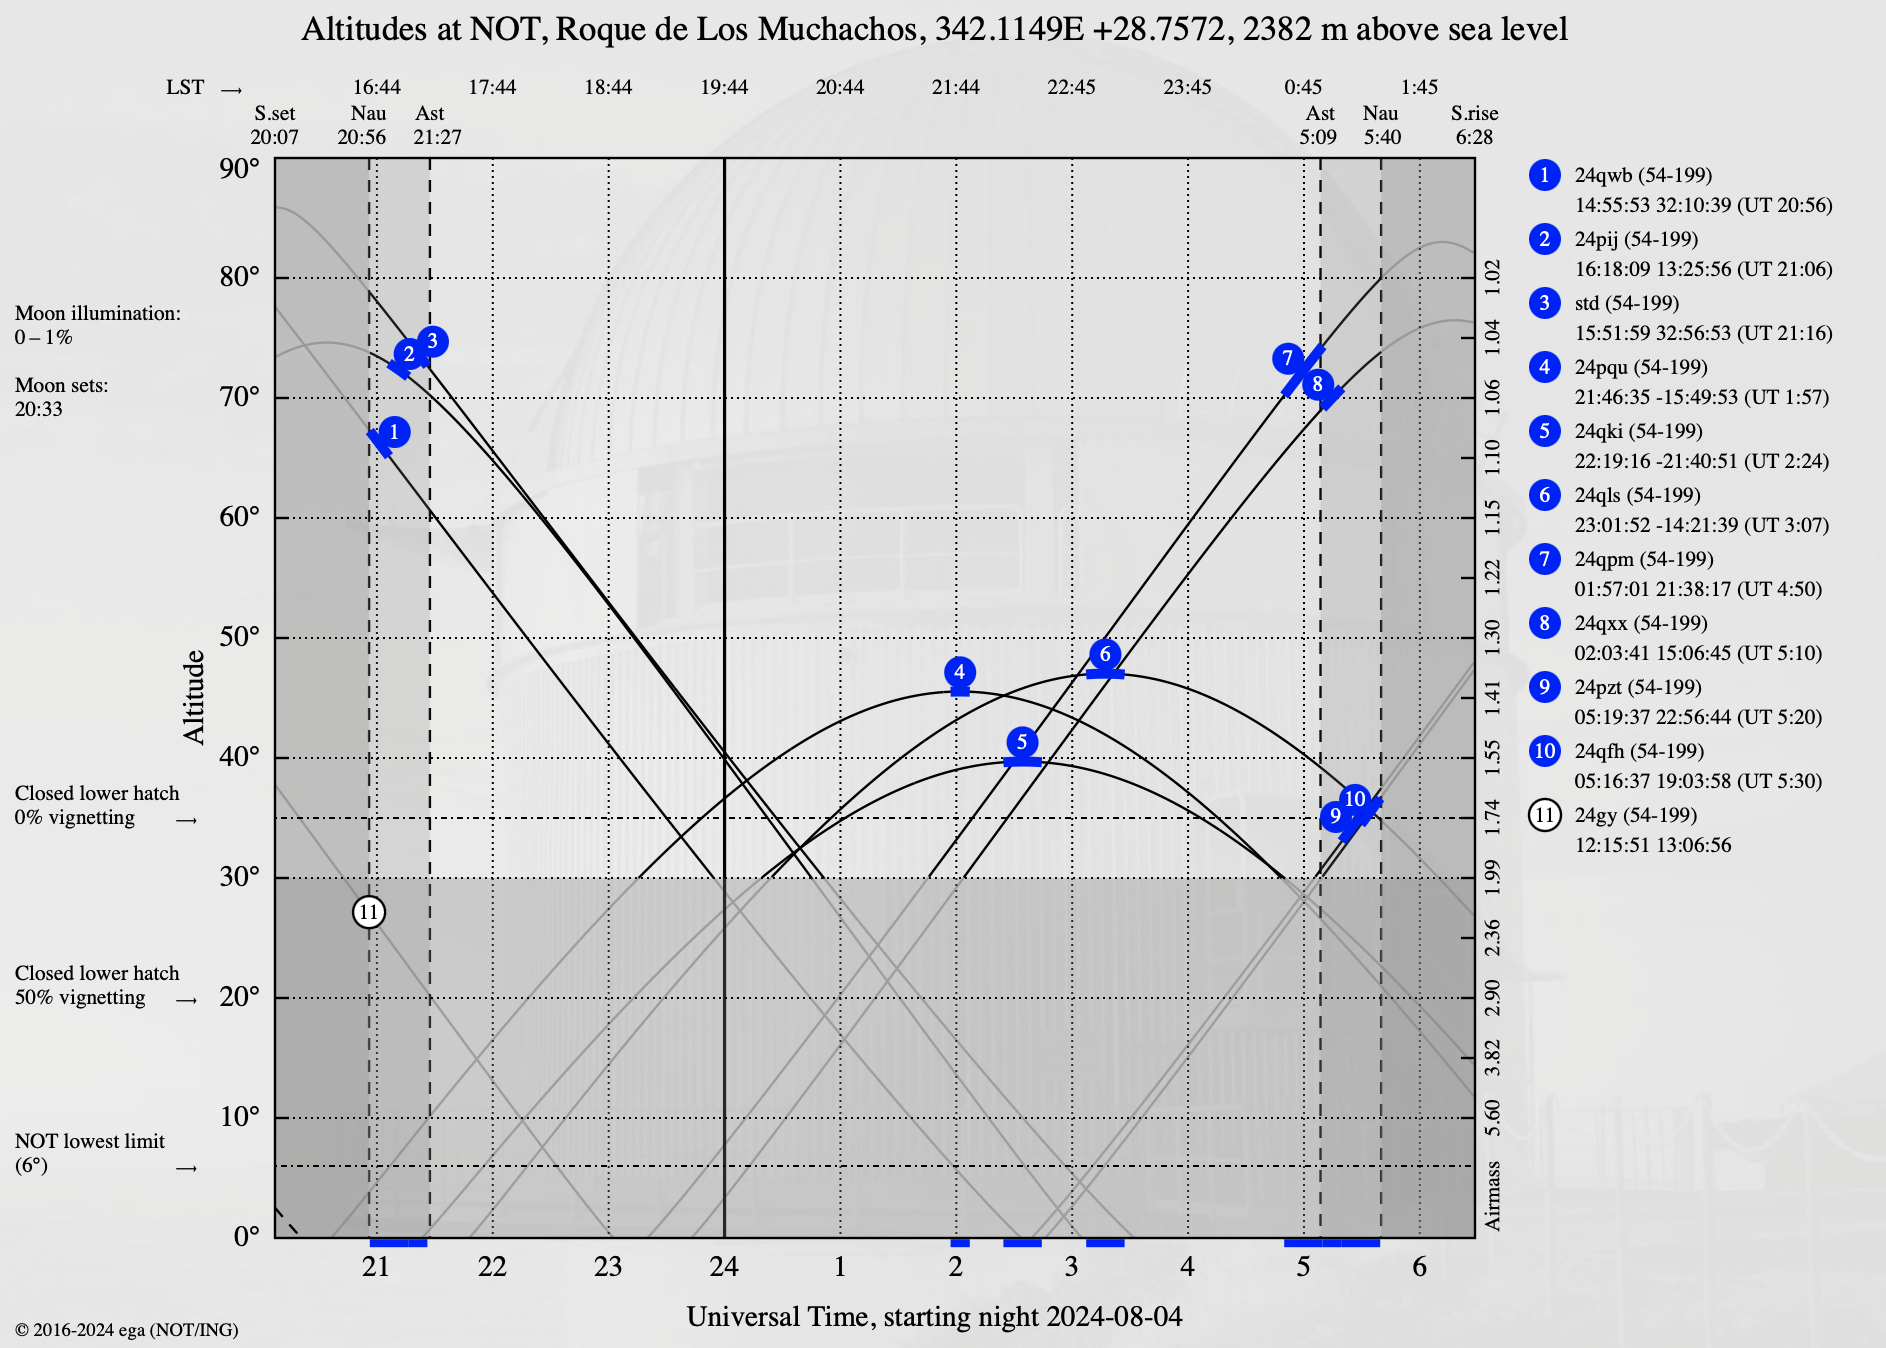
\includegraphics[width=\textwidth]{../Images/chapter_2/visplot.png}
    \caption{Night plan for the NOT on the night of 10 August 2024. Targets are plotted with their altitude as a function of universal standard time. Local stellar time is shown on top. The target priority has been colour-coded, with the coloured bars showing the amount of time each observation is expected to take. Green targets have already been completed, and the red vertical line shows the current time. Several unscheduled backup targets are shown in case the plan has to be updated during the night.}
    \label{visplot}
\end{figure}

\end{document}